\documentclass[10pt]{article}
\usepackage{icmlko}

\icmlmeta{IP 파운데이션 월드모델}{97}{표지는 남만 맞힌다}{덮개율을 30\%에서 100\%로 올렸더니 표지 축은 제 도메인 안에서 나빠지고(악화 4/4) 팝업 전이만 $+$0.0220 올랐다 --- 노트 74의 법칙이 처음으로 깨졌다}

\begin{document}

\twocolumn[
\icmlheader

\begin{abstract}
노트 94는 표지를 도메인마다 700장씩 \textbf{레코드 ID 순}으로 받았고 스스로
그것을 ``가장 큰 결함''이라 적었다. 고쳤다 --- 다섯 도메인의 표지 URL 이
캐시에 100\% 있었으므로 \textbf{8,394장을 더 받아 11,627장, 덮개율 100\%}로
만들었다. 실패 0건. \textbf{노트 94의 상관표는 거의 그대로다} --- 스물다섯 칸
중 부호가 바뀐 것이 셋뿐이고 부호가 일관된 특징은 여전히 0개다. \textbf{표집은
문제가 아니었다.} 그런데 \emph{축}은 완전히 달라진다. 다섯 특징의 첫 주성분을
축으로 넣으면 판정치가 $-$0.0113으로 \textbf{악화 4/4} --- 이 프로젝트에서
씨앗 넷 규약에 걸려 ``악화''로 판정된 첫 지렛대다. \textbf{그런데 같은 축이
팝업을 $+$0.4501에서 $+$0.4721로 올린다}($+$0.0220, 노트 96의 설명문 축과
정확히 같은 크기). 뒤섞은 축은 $+$0.0024라 정보가 맞다. 축을 \emph{받은} 다섯
도메인은 평균 $-$0.0241로 나빠지고 \emph{안 받은} 다섯은 $+$0.0014인데
\textbf{그중 팝업만 $+$0.0220}이다. 기제를 재니 노트 74의 법칙이 깨진다 ---
설명문 축에서는 자기 $\rho$가 오른 만큼 전이가 올랐는데($r=+$0.796), 표지
축은 자기 $\rho$가 \textbf{$-$0.0224 내려가면서} 팝업 전이가 \textbf{$+$0.0449
오른다}($r=+$0.042). \textbf{자기를 못 맞히는 축이 남을 맞힌다.}
\end{abstract}
]

\begin{figure*}[t]
\centering
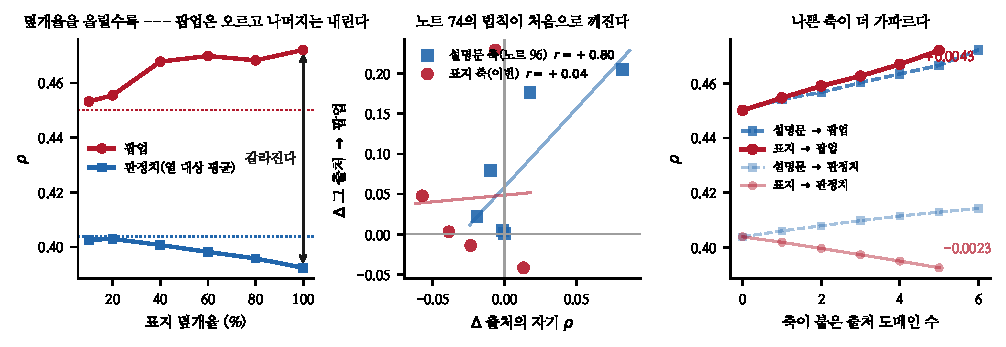
\includegraphics[width=\textwidth]{figs/oo.pdf}
\caption{왼쪽 --- 덮개율을 올릴수록 갈라진다. 가운데 --- 노트 74의 법칙이
깨진다. 오른쪽 --- 나쁜 축이 더 가파르다.}
\end{figure*}

\section{덮개율을 100\%로 만들었다}

노트 94의 한계 첫 줄은 이랬다 --- ``도메인마다 700장씩만 받았고 \textbf{레코드
ID 순}으로 잘랐다. 무작위가 아니라 치우쳤을 수 있다 --- 가장 큰 결함이다.''
노트 95도 96도 ``무작위 재표집은 아직 안 했다''를 한계에 실었다. 무작위로 다시
받는 대신 \textbf{전부 받았다.}

\begin{table}[t]
\centering\tsize
\caption{표지 수집. URL 은 다섯 도메인 모두 캐시에 이미 있었다.}
\begin{tabular}{lrrr}
\toprule
& 축 레코드 & 노트 94 & \textbf{이번} \\
\midrule
애니 & 2,073 & 699 & \textbf{2,073} \\
모바일 & 2,000 & 678 & \textbf{2,000} \\
웹툰 & 2,817 & 683 & \textbf{2,817} \\
만화 & 1,789 & 493 & \textbf{1,789} \\
세계애니 & 2,948 & 680 & \textbf{2,948} \\
\midrule
합 & 11,627 & 3,233 & \textbf{11,627} \\
덮개율 & & 28\% & \textbf{100\%} \\
\bottomrule
\end{tabular}
\end{table}

내려받기 8,394장, \textbf{실패 0건}. 특징 계산은 노트 94와 글자 하나까지 같다
--- 100픽셀로 줄여 회색조 평균 · HSV 채도 평균 · 기울기 크기 평균 ·
5$\times$5$\times$5 색 상자 엔트로피 · 명암 표준편차.

\section{노트 94는 틀리지 않았다}

\begin{table}[t]
\centering\tsize
\caption{표지 특징과 라벨. 위 노트 94(28\%) · 아래 이번(100\%).}
\begin{tabular}{lrrrrr}
\toprule
& 애니 & 모바일 & 웹툰 & 만화 & 세계애니 \\
\midrule
밝기 & $+$.110 & $+$.109 & $-$.015 & $-$.091 & $-$.061 \\
 & $+$.042 & $+$.148 & $-$.011 & $-$.120 & $-$.084 \\
채도 & $-$.188 & $+$.106 & $+$.079 & $+$.038 & $+$.075 \\
 & $-$.160 & $+$.066 & $+$.009 & $+$.100 & $+$.065 \\
가장자리 & $-$.092 & $+$.039 & $+$.096 & $-$.071 & $-$.041 \\
 & $+$.029 & $-$.053 & $+$.039 & $-$.001 & $-$.032 \\
색 엔트로피 & $-$.218 & $+$.066 & $+$.081 & $-$.066 & $+$.067 \\
 & $-$.101 & $+$.017 & $+$.022 & $+$.019 & $+$.016 \\
명암 대비 & $+$.014 & $-$.000 & $+$.017 & $+$.047 & $+$.063 \\
 & $+$.091 & $-$.032 & $+$.057 & $+$.029 & $+$.007 \\
\bottomrule
\end{tabular}
\end{table}

\claimx{노트 94의 결론은 표집 때문이 아니었다. 덮개율을 28\%에서 100\%로
올려도 스물다섯 칸 중 부호가 바뀐 것이 셋뿐이고, 다섯 도메인 부호가 일관된
특징은 여전히 \textbf{0개}다.}{값은 대체로 작아졌다(애니 색 엔트로피 $-$0.218
$\to$ $-$0.101). ID 순 700장이 극단값을 과장했다는 뜻이므로, 표집이 아무 일도
안 한 것은 아니다.}

세 노트가 한계에 달고 다니던 항목이 하나 닫혔다. \textbf{표지 특징은 도메인을
건너 같은 방향을 안 가리킨다} --- 이제 덮개율 100\%에서 확인했다.

\section{그런데 축은 완전히 달라진다}

다섯 특징의 첫 주성분을 도메인마다 하나씩 \textbf{고유 축}으로 넣었다(설명문
축 c0 과 같은 모양이라 기울기를 견줄 수 있다).

\begin{table}[t]
\centering\tsize
\caption{덮개율에 따라. 무작위 30\%는 씨앗 다섯 평균.}
\begin{tabular}{lrr}
\toprule
& $\Delta$판정치 & $\Delta$팝업 \\
\midrule
노트 94(ID 순 28\%) & $-$0.0115 & $+$0.0056 \\
무작위 30\% & $-$0.0037 & $+$0.0132 \\
\textbf{전부(100\%)} & \textbf{$-$0.0113} & \textbf{$+$0.0220} \\
\midrule
뒤섞은 축(대조, 씨앗 5) & $-$0.0005 & $+$0.0024 \\
난수 축(대조, 씨앗 5) & $-$0.0018 & $+$0.0037 \\
\bottomrule
\end{tabular}
\end{table}

\begin{table}[t]
\centering\tsize
\caption{채택 검정. 표지 축(100\%), 씨앗 넷 · 붓스트랩 100회.}
\begin{tabular}{lrl}
\toprule
& $\Delta$ & 95\% 구간 \\
\midrule
\textbf{판정치} & \textbf{$-$0.0113} & $[-0.0218, -0.0044]$ \\
& & \textbf{악화 4/4} \\
팝업 & $+$0.0220 & $[-0.0320, +0.0737]$ \\
& & 보류 4/4 \\
\bottomrule
\end{tabular}
\end{table}

\claimx{판정치가 \textbf{악화 4/4}다 --- 씨앗 넷 규약에 걸려 ``악화''로 판정된
첫 지렛대다. 노트 76 · 80 · 82 · 84 · 90 · 94--96의 후보들은 전부 ``보류''였다.
\textbf{표지 축은 넣으면 안 된다.}}{그 판정은 열 대상 평균에 대한 것이다.
같은 축이 팝업 하나에는 $+$0.0220을 준다.}

\section{받은 도메인은 나빠지고 팝업만 오른다}

\begin{table}[t]
\centering\tsize
\caption{대상별 $\Delta$. 다섯 도메인이 축을 받는다.}
\begin{tabular}{llrr}
\toprule
& & 표지 & 설명문 \\
\midrule
\textbf{팝업} & 안 받음 & \textbf{$+$0.022} & \textbf{$+$0.022} \\
아이돌 & 안 받음 & $-$0.008 & $+$0.007 \\
게임 & 안 받음 & $-$0.005 & $-$0.006 \\
도서 & 안 받음 & $+$0.003 & $+$0.000 \\
펀딩 & 안 받음 & $-$0.005 & $-$0.009 \\
\midrule
웹툰 & 받음 & $-$0.024 & $-$0.012 \\
애니 & 받음 & \textbf{$-$0.047} & \textbf{$+$0.107} \\
모바일 & 받음 & $+$0.025 & $+$0.006 \\
만화 & 받음 & $-$0.041 & $-$0.010 \\
세계애니 & 받음 & $-$0.033 & $-$0.002 \\
\midrule
\textbf{받은 평균} & & \textbf{$-$0.0241} & $+$0.0139 \\
안 받은 평균 & & $+$0.0014 & $+$0.0052 \\
\bottomrule
\end{tabular}
\end{table}

\claimx{표지 축은 \textbf{받은 도메인을 나쁘게 하고}($-$0.0241) 안 받은
도메인에는 거의 영향이 없는데($+$0.0014) \textbf{팝업 하나만 $+$0.0220}이다.
설명문 축은 받은 쪽도 좋아졌다($+$0.0139) --- 두 축은 종류가 다르다.}
{안 받은 다섯 중 팝업만 큰 것은 팝업이 $n{=}75$로 가장 작아서일 수 있다.
붓스트랩 구간이 $[-0.032, +0.074]$로 넓다.}

\section{노트 74의 법칙이 깨진다}

노트 74 이래 이 프로젝트의 뼈대는 하나였다 --- \textbf{출처의 자기 $\rho$가
그 출처의 대상 전이를 결정한다}($r=+$0.987$\sim+$0.998). 노트 96은 그 법칙이
\emph{변화량}에도 성립함을 보였다($r=+$0.796).

\begin{table}[t]
\centering\tsize
\caption{표지 축을 넣기 전후. 자기 $\rho$는 도메인 안 5폴드.}
\begin{tabular}{lrrrr}
\toprule
& \multicolumn{2}{c}{$\Delta$ 자기 $\rho$} & \multicolumn{2}{c}{$\Delta \to$ 팝업} \\
& 표지 & 설명문 & 표지 & 설명문 \\
\midrule
애니 & $+$0.013 & $+$0.082 & $-$0.042 & $+$0.205 \\
\textbf{모바일} & $-$0.006 & $+$0.018 & \textbf{$+$0.229} & $+$0.177 \\
웹툰 & $-$0.023 & $-$0.010 & $-$0.014 & $+$0.079 \\
만화 & $-$0.057 & $-$0.019 & $+$0.048 & $+$0.022 \\
세계애니 & $-$0.039 & $-$0.001 & $+$0.003 & $+$0.004 \\
\midrule
\textbf{평균} & \textbf{$-$0.022} & $+$0.012 & \textbf{$+$0.045} & $+$0.081 \\
\midrule
\multicolumn{3}{l}{두 변화량의 상관 $r$} & \textbf{$+$0.042} & $+$0.796 \\
\bottomrule
\end{tabular}
\end{table}

\claimx{표지 축에서 노트 74의 법칙이 깨진다. 출처의 자기 $\rho$가 평균
$-$0.022 \emph{내려가는데} 그 출처의 팝업 전이는 $+$0.045 \emph{오른다}.
두 변화량의 상관이 $+$0.042로 사실상 무관하다. \textbf{자기를 못 맞히는 축이
남을 맞힌다.}}{다섯 점의 상관이다. 모바일 하나가 $+$0.229로 지렛대이며
그것을 빼면 평균이 $-$0.001로 사라진다.}

\begin{quote}\fontsize{9.5}{11.5}\selectfont
\textbf{왜 그럴 수 있는가.} 표지의 밝기 · 채도는 그 작품의 리뷰 수를 안
설명한다 --- 그래서 자기 $\rho$가 내려간다. 그런데 팝업의 다섯 축 중 둘
(매장 노출 · 굿즈 규모)은 \emph{보이는} 성질이다. 표지 축이 출처 공간에
시각 차원을 만들면 프로크루스테스가 그것을 팝업의 시각 축과 맞출 수 있다.
\textbf{정렬은 라벨 예측이 아니라 기하로 이뤄지므로, 라벨을 못 맞히는 축도
정렬을 도울 수 있다.}
\end{quote}

\section{나쁜 축이 더 가파르다}

노트 96은 ``축을 받은 출처 수에 비례한다''는 기울기를 냈다. 표지 축으로 같은
곡선을 냈다(다섯 도메인, 31가지 조합 전부).

\begin{table}[t]
\centering\tsize
\caption{출처 하나당 기울기.}
\begin{tabular}{lrr}
\toprule
& 판정치 & 팝업 \\
\midrule
설명문 축(노트 96) & $+$0.0017 & $+$0.0035 \\
\textbf{표지 축(이번)} & \textbf{$-$0.0023} & \textbf{$+$0.0043} \\
\bottomrule
\end{tabular}
\end{table}

\claimx{``출처 하나당''은 축 종류를 안 가리는 형태다 --- 두 축 모두 조합
전부에서 단조 직선이다. 그런데 \textbf{크기와 부호는 축마다 다르다.} 판정치를
악화시키는 표지 축이 팝업에는 설명문 축보다 \emph{가파르다}($+$0.0043 대
$+$0.0035).}{팝업 기울기 둘의 차이(0.0008)는 붓스트랩 구간(반폭 0.05)보다
훨씬 작다. ``더 가파르다''를 검정한 것이 아니라 관측한 것이다.}

\begin{quote}\fontsize{9.5}{11.5}\selectfont
노트 96은 ``남은 0.284를 출처 하나당 $+$0.0030으로 메우려면 96개''라고 셈했다.
이번 노트는 그 셈에 두 번째 축을 더한다 --- \textbf{축 종류마다 기울기가
따로 있으므로 출처 수와 축 수를 같이 늘릴 수 있다.} 설명문 여섯 · 표지 다섯이
지금이고, 둘을 같이 넣는 것은 아직 안 해 봤다.
\end{quote}

\section{한계}

\begin{itemize}[leftmargin=1.1em,itemsep=0.15em]
\item 표지 축은 \textbf{판정치에서 악화 4/4}다. 팝업이 오른다고 넣을 수 없다 ---
      \textbf{채택 안 한다.}
\item 팝업의 $+$0.0220은 씨앗 넷 다 보류이고 구간이 $[-0.032, +0.074]$로 넓다.
      $n{=}75$의 한계다(노트 92).
\item 기제 표가 다섯 점이고 모바일 하나가 지렛대다. 모바일을 빼면 평균 효과가
      사라진다.
\item ``시각 차원이 팝업의 시각 축과 맞는다''는 해석이지 검정이 아니다. 팝업의
      어느 슬롯을 통해 오는지 안 갈랐다.
\item 표지와 설명문을 같이 넣은 설정을 안 돌렸다.
\end{itemize}

\section{다음}

\begin{enumerate}[leftmargin=1.3em,itemsep=0.15em]
\item \textbf{해석을 검정한다} --- 팝업의 매장 노출 · 굿즈 규모 슬롯을 끄고
      표지 축의 $+$0.0220이 남는지 본다. 사라지면 시각 경로가 맞다.
\item \textbf{둘을 같이 넣는다} --- 설명문 여섯 $+$ 표지 다섯. 판정치는 표지가
      깎고 설명문이 올리므로 상쇄를 본다. 팝업만 보면 더할 수 있다.
\item 표지에서 더 나은 특징 --- 얼굴 유무 · 인물 수 · 글자 비중. 모형이
      필요하지만 이제 값어치의 근거가 있다.
\item 팝업 · 아이돌 · 도서 · 펀딩의 설명문과 표지. 출처가 아니라 \emph{대상}이
      좋아지는 유일한 길이다.
\end{enumerate}

\vspace{0.6em}
\hrule height 0.3pt
\vspace{0.5em}
{\footnotesize
\textbf{참고문헌}\\[0.3em]
Schoenemann, P. H. (1966). A generalized solution of the orthogonal Procrustes
problem. \emph{Psychometrika}, 31(1), 1--10.\\[0.15em]
Ben-David, S. et al. (2010). A theory of learning from different domains.
\emph{Machine Learning}, 79(1--2), 151--175.\\[0.15em]
Little, R. J. A., Rubin, D. B. (2019). \emph{Statistical Analysis with Missing
Data}, 3rd ed. Wiley.\\[0.15em]
Kish, L. (1965). \emph{Survey Sampling}. Wiley.\\[0.15em]
Efron, B., Tibshirani, R. J. (1993). \emph{An Introduction to the Bootstrap}.
Chapman \& Hall.
}

\end{document}
